\documentclass[conference]{IEEEtran}
\IEEEoverridecommandlockouts

\usepackage[utf8]{inputenc}
\usepackage[T1]{fontenc}
\usepackage{graphicx}
\usepackage{booktabs}
\usepackage{url}
\usepackage{amsmath}

\hyphenation{report historical}

\title{Aegis: Milestone-Based Crowdfunding on Ethereum with Contribution-Weighted Voting}

\author{\IEEEauthorblockN{Rifqi Ramadhan, George Wiliam Thomas Gonata, Samuel Tanaka Sibarani, and Riri Fitri Sari}
\IEEEauthorblockA{Department of Electrical Engineering, Faculty of Engineering, University of Indonesia\\
Email: {\tiny \texttt{rifqi.ramadhan22@ui.ac.id}, \texttt{george.william@ui.ac.id},}\\
{\tiny \texttt{samuel.tanaka@ui.ac.id}, \texttt{riri@ui.ac.id}}}}

\begin{document}
\maketitle

\begin{abstract}
Aegis, a blockchain-enabled decentralized crowdfunding concept to be built on the work of Ethereum, introduced post-campaign accountability through contribution-weighted voting on project milestones. Unlike traditional centralized crowdfunding platforms that release funds in bulk immediately after a campaign ends, Aegis locks the raised capital in a project-specific smart contract escrow. The funds are then conditionally released to the creator in tranches, each corresponding to a specific project milestone. Creators must submit detailed progress reports (stored as metadata), which backers review and vote upon. Backers' voting weights are proportional to their financial exposure (ETH contribution). If a milestone report is approved by a majority, the allocated tranche is released; if rejected, or if the project is cancelled, backers can claim proportional refunds from the remaining contract balance. We implement the core contracts (Factory and Project) and a React-based frontend application integrated with MetaMask. The results show that the platform successfully maintains correctness in state transitions and refund processes on a local Hardhat network, as verified through comparison with the industry-standard Juicebox Protocol and academic hybrid blockchain-AI architectures.
\end{abstract}

\begin{IEEEkeywords}
Blockchain, Crowdfunding, Smart Contract, Ethereum, Milestone Funding, Web3, Contribution-Weighted Voting
\end{IEEEkeywords}

\section{Introduction}

\subsection{Problem Definition}
Crowdfunding has emerged as a powerful mechanism to democratize capital raising, allowing creators to fund projects through small contributions from a global base of backers. However, traditional centralized platforms (e.g., Kickstarter, GoFundMe) face severe limitations in transparency, fund governance, and post-campaign accountability. Once a project successfully meets its funding goal, the accumulated capital is typically transferred in bulk to the creator. Backers are left with virtually no control over how funds are spent, and project abandonment or misuse of funds is common. This creates a classic principal-agent problem where the incentives of the project creator (agent) diverge from those of the backers (principals) once the funding phase concludes.

\subsection{Blockchain Need Analysis}
To address these challenges, a decentralized approach using blockchain technology and smart contracts is required. Blockchain is uniquely suited to solve the crowdfunding trust deficit due to the following characteristics:
\begin{itemize}
	\item \textbf{Decentralized Escrow}: Smart contracts can act as neutral, programmatically controlled escrows that lock contributions without depending on a trusted centralized intermediary.
	\item \textbf{Immutability and Auditability}: Every contribution, report submission, and vote is recorded immutability on-chain, providing a transparent ledger that prevents historical tampering.
	\item \textbf{Automated Rule Execution}: Rules governing fund release, voting periods, and refunds are executed deterministically and programmatically, removing human bias or central platform intervention.
\end{itemize}
Nonetheless, simply migrating traditional bulk-release crowdfunding models to the blockchain does not solve the post-campaign principal-agent problem. Creators can still withdraw all funds and abandon the project, leaving backers with no recourse. Hence, blockchain technology is a necessary but not sufficient foundation; it must be coupled with a milestone-based enforcement mechanism.

\subsection{Innovation of Aegis}
This paper presents Aegis, a decentralized crowdfunding platform concept designed to bridge the post-campaign trust gap. The core innovation of Aegis lies in its integration of a milestone-locked escrow contract with a contribution-weighted voting model. 

Before initiating their campaigns, project creators must define a structured set of milestones with associated funding tranches. The contributed capital, denominated in Ether (ETH), is locked securely in a dedicated smart contract. To unlock each tranche, the creator must submit a progress report containing proof of work. Backers then vote to approve or reject the report, with their voting weights determined by their individual contributions. This aligns voting power directly with backers' financial risk, mitigating the risk of Sybil attacks and ensuring that decision-making authority matches capital exposure.

The key contributions of this paper are summarized as follows:
\begin{itemize}
	\item A contribution-weighted voting model that aligns voting power directly with backers' financial risk and provides Sybil resistance.
	\item An end-to-end decentralized application (DApp) architecture including factory-deployed project contracts and a React user interface connected via MetaMask.
	\item A rigorous state-machine model that governs project lifecycles (Funding, Active, Completed, Cancelled) to prevent invalid state transitions.
	\item A comparative analysis of Aegis against both the commercial Juicebox Protocol and research-oriented hybrid blockchain-AI architectures.
\end{itemize}

The rest of this paper is structured as follows: Section II reviews related work. Section III explains the proposed contribution-weighted voting method. Section IV details the system design and architecture. Section V presents the implementation details. Section VI evaluates the platform concept through test scenarios and discusses limitations. Finally, Section VII concludes the paper and outlines future research.

\section{Related Work}

\subsection{Juicebox Protocol (Commercial Industry)}
The Juicebox Protocol is a widely used decentralized treasury management and crowdfunding platform on Ethereum \cite{juicebox}. It allows communities to configure funding cycles, issue tokens, and manage treasury redemptions. Juicebox is highly flexible and scalable for crowdfunding and blockchain DAOs, as it automates token issuance, treasury payouts, and multi-destination allocations across configurable funding cycles, thereby reducing operational overhead. However, it focuses primarily on continuous funding and tokenomics rather than structured milestone enforcement. In Juicebox, fund release is generally governed by fixed cycle configurations or open-ended multisig allocations. There is no built-in, out-of-the-box mechanism that directly ties fund tranches to backer-reviewed milestone reports, which limits its applicability for projects requiring strict, phased accountability.

\subsection{Academic Blockchain Crowdfunding Systems}
In academic literature, several researchers have proposed using Ethereum-based smart contracts to improve trust and mitigate fraud in crowdfunding. Rathore and Rizvi \cite{rathore2023decentralized} explored a basic decentralized crowdfunding platform on blockchain, highlighting the advantages of smart contracts in removing centralized intermediaries and reducing transaction fees. Similarly, Jayapal, Xavier, and Arunachalam \cite{jayapal2023capitalizing} examined the efficiency of Ethereum smart contracts in automating campaign workflows, ensuring that creators receive funds only if the target is met, thereby reducing financial risk for backers.

To address information asymmetry, Ahmad and Rahman \cite{ahmad2021applying} proposed applying smart contracts to increase trust by keeping all transaction and project statuses fully transparent. Aprialim, Adnan, and Paundu \cite{aprialim2021penerapan} presented a smart contract integration model that focuses on structural security during the funding phase. Furthermore, BitFund \cite{bitfund2020} modeled an open-ended crowdfunding framework designed for smart and connected nations, emphasizing public ledger auditing. 

However, these models primarily focus on the pre-campaign and active campaign phases, leaving post-campaign milestones unmanaged. Once the funding goal is met, these architectures disperse funds directly, failing to solve the problem of subsequent project abandonment.

\subsection{Decentralized Escrow and Governance Models}
To protect funds post-campaign, some systems incorporate escrow and governance structures. Shelke et al. \cite{shelke2022blockchain} proposed a decentralized escrow framework that locks contributions and allows manual intervention by backers, although it lacks a structured milestone workflow. Zichichi et al. \cite{zichichi2019likestarter} developed LikeStarter, a smart contract-based social DAO that utilizes social proof and voting to align incentive structures between creators and backers. 

Periodic milestone payments were formally modeled by Alruwaili and Kruger \cite{alruwaili2020milestone}, who proposed utilizing fair e-voting systems to approve tranches sequentially. While their model is mathematically robust, it relies on complex cryptographic voting schemes that are difficult to deploy on-chain due to gas constraints. Aegis simplifies this by implementing a contribution-weighted simple majority voting system directly in the project contract, which is gas-efficient and easily integrated with a standard Web3 interface. 

To validate the security of these complex workflows, Villanueva, Srinivasan, and Rehman \cite{villanueva2025metamorphic} proposed metamorphic testing techniques to detect potential logical vulnerabilities in Ethereum-based crowdfunding contracts. Chen et al. \cite{chen2023dcc} discussed decentralized co-governance models to improve long-term project sustainability, emphasizing the importance of collaborative oversight.

Table~\ref{tab:comparison} highlights the key differences between Aegis and these related solutions, showing that Aegis occupies a unique niche by providing a practical, end-to-end DApp with robust, contribution-weighted milestone voting, which can be extended to other use cases such as decentralized grant distributions, public goods funding, and service-level agreement (SLA) verifications.

\begin{table}[t]
\centering
\caption{Comparison of Aegis with Related Solutions}
\label{tab:comparison}
\begin{tabular}{lccc}
\toprule
\textbf{Criterion} & \textbf{Juicebox \cite{juicebox}} & \textbf{Hybrid AI \cite{hybridai}} & \textbf{Aegis} \\
\midrule
Ethereum-based & Yes & Yes & Yes \\
Milestone management & Limited & Yes & Yes \\
Community voting & Limited & Limited & Yes \\
Automatic fund release & Partial & Yes & Yes \\
AI verification & No & Yes & No \\
End-to-end DApp & Yes & No & Yes \\
\bottomrule
\end{tabular}
\end{table}

\section{Proposed Method}
Aegis addresses post-campaign risk through a novel, contribution-weighted milestone voting mechanism. The system requirements and voting dynamics are formalized below.

\subsection{Contribution-Weighted Voting Model}
Let $P$ be a crowdfunding project with a total funding goal $G$ and a set of backers $B = \{1, 2, \dots, n\}$. Each backer $i \in B$ contributes an amount of Ether $c_i > 0$ such that the total funded amount $C_{\text{total}}$ satisfies:
\begin{equation}
C_{\text{total}} = \sum_{i=1}^{n} c_i \ge G
\end{equation}
A project is structured into a set of sequential milestones $M = \{M_1, M_2, \dots, M_m\}$, where each milestone $M_j$ has an allocated funding tranche $A_j > 0$ such that:
\begin{equation}
\sum_{j=1}^{m} A_j = G
\end{equation}

When the creator submits progress proof for milestone $M_j$, backers can cast votes $v_{i,j} \in \{\text{Approve}, \text{Reject}\}$. The voting weight $w_i$ of backer $i$ is defined as their financial contribution:
\begin{equation}
w_i = c_i
\end{equation}
Let $V_Y$ be the sum of weights of backers who voted to approve, and $V_N$ be the sum of weights of backers who voted to reject:
\begin{equation}
V_Y = \sum_{i \in B, v_{i,j} = \text{Approve}} w_i, \quad V_N = \sum_{i \in B, v_{i,j} = \text{Reject}} w_i
\end{equation}
Milestone $M_j$ is approved if the approval weight reaches a simple majority of the total project funding:
\begin{equation}
V_Y > \frac{C_{\text{total}}}{2}
\end{equation}
Upon approval, the tranche $A_j$ is released to the creator's wallet. If $V_N > C_{\text{total}}/2$, the milestone is rejected, which halts the project and allows backers to claim refunds.

\subsection{Discussion of Voting Design and Sybil Resistance}
The choice of a contribution-weighted voting model addresses several critical challenges in decentralized governance:
\begin{itemize}
	\item \textbf{Sybil Attack Mitigation}: Standard blockchain systems that implement a one-address-one-vote rule are highly vulnerable to Sybil attacks, where an individual creates multiple Ethereum addresses to manipulate outcomes. By tying voting power directly to contributed ETH ($w_i = c_i$), Aegis ensures that voting weight is bound to capital locked in the contract, rendering Sybil attacks ineffective.
	\item \textbf{Incentive Alignment}: Linking vote weights to contributions aligns decision-making authority with financial exposure. Backers who have funded a larger portion of the project goal carry higher financial risk and thus command a larger voice in progress validation.
	\item \textbf{Instant Finalization vs. Timeout}: To optimize operational efficiency, the contract evaluates consensus dynamically during each vote. If the total yes votes ($V_Y$) or no votes ($V_N$) exceed the absolute majority threshold ($C_{\text{total}}/2$), the voting process is finalized instantly, and funds are either released or frozen. If no majority is reached, the vote remains open until the expiration of the voting period ($T_{\text{voting}} = 7$ days), after which the milestone status is determined by simple majority.
\end{itemize}

\subsection{Refund Mechanism}
If the project is cancelled by the creator, or if a milestone is rejected by backers, the project transitions to the \textit{Cancelled} state. Backers are eligible to claim a refund proportional to their contribution from the remaining contract balance $R$. The refund amount $R_i$ for backer $i$ is calculated as:
\begin{equation}
\label{eq:refund}
R_i = c_i \times \frac{R}{C_{\text{total}} - C_{\text{released}}}
\end{equation}
where $C_{\text{released}}$ is the total amount of funds already released to the creator for approved milestones. This formulation ensures that remaining, unreleased funds are returned to backers fairly, taking into account any tranches already dispersed for successfully completed work.

\section{System Design}

\subsection{Architecture Overview}
The Aegis platform uses a decentralized topology consisting of three layers: the Client Interface (React DApp), the Web3 Provider (MetaMask wallet), and the Ethereum Smart Contracts. Figure~\ref{fig:usecase} illustrates the core use case view of the platform.

\begin{figure}[h]
\centering
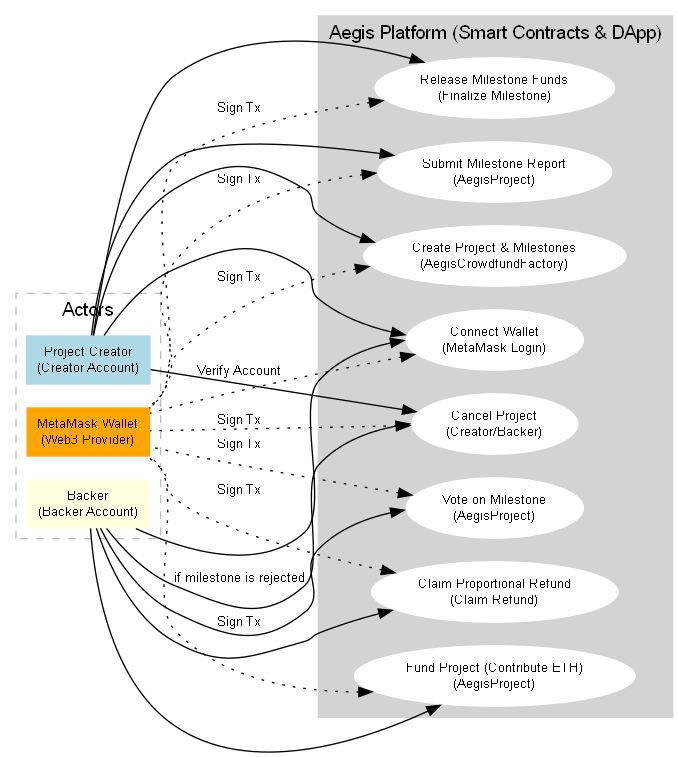
\includegraphics[width=0.75\columnwidth]{../use-case-en.png}
\caption{Use case view of Aegis actors and core actions.}
\label{fig:usecase}
\end{figure}

The topology follows a factory-project pattern:
\begin{enumerate}
	\item \textbf{AegisCrowdfundFactory}: A single, registry contract deployed on-chain that creators interact with to deploy individual projects. This reduces deploy-time gas overhead and provides a centralized index of all campaigns.
	\item \textbf{AegisProject}: An independent, self-contained escrow contract deployed for each campaign. It manages the campaign's lifecycle, secures contributed ETH, records milestones, handles voting, and disperses funds.
\end{enumerate}

\subsection{Data Entities and Mappings}
To enforce governance rules efficiently, the \texttt{AegisProject} smart contract maintains three primary data mapping structures in state storage:
\begin{itemize}
	\item \texttt{contributions (address => uint256)}: Maps each backer's address to the amount of ETH they contributed. This serves as the source of truth for both refund disbursements and voting weights.
	\item \texttt{hasVoted (address => mapping(uint256 => bool))}: A nested mapping that tracks whether a specific backer has already cast a vote on a given milestone ID, preventing double-voting.
	\item \texttt{milestones (Milestone[])}: An ordered array of `Milestone` structs containing description, amount, status, and progress reports.
\end{itemize}

\subsection{Workflow Sequence}
Figure~\ref{fig:sequence} depicts the chronological sequence of interactions between the user, the DApp frontend, MetaMask, and the smart contracts during milestone reporting and voting.

\begin{figure}[h]
\centering
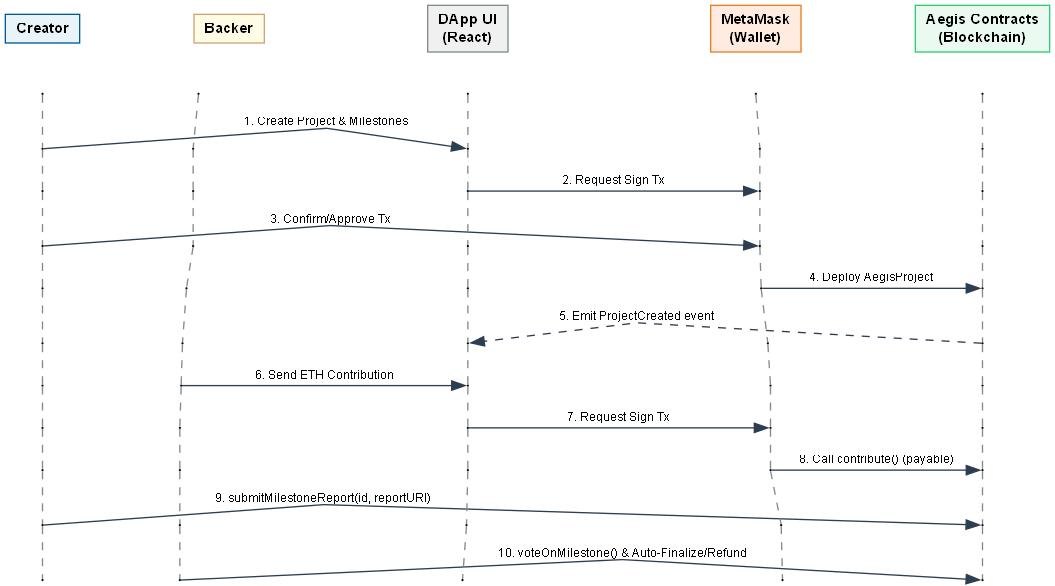
\includegraphics[width=0.9\columnwidth]{../sequence-en.png}
\caption{Sequence of UI-wallet-contract interactions for milestone approval.}
\label{fig:sequence}
\end{figure}

First, the creator submits milestone proof. The frontend captures this data and calls the contract's `submitMilestoneReport` function, prompting MetaMask to sign the transaction. Once confirmed, backers can query the report and cast their vote via `voteOnMilestone`. The contract counts the weights and automatically releases the tranche if a majority is met, or updates status to allow finalization after the voting period ends.

\subsection{Project Lifecycle State Machine}
The `AegisProject` contract implements a strict finite state machine (FSM) to prevent reentrancy and out-of-order execution. The states are defined as follows:
\begin{itemize}
	\item \textbf{Funding}: The initial state where backers contribute ETH. If the goal $G$ is reached before the deadline, it transitions to \textit{Active}. If the deadline passes without meeting $G$, it transitions to \textit{Cancelled}, enabling refunds.
	\item \textbf{Active}: The project is funded. The creator can submit milestone reports, and backers vote.
	\item \textbf{Completed}: Transitions here automatically when all milestones have been successfully approved and all funds released.
	\item \textbf{Cancelled}: Triggered by funding failure, creator cancellation, or milestone rejection. All remaining funds are frozen in escrow, and backers can withdraw their proportional refunds.
\end{itemize}

\section{Implementation}
This section describes the practical implementation of the Aegis platform. The codebase is organized into two primary layers: the smart contracts representing the backend blockchain logic, and the React-based decentralized frontend application. The process of integrating these components relies on Web3 providers to establish a joint communication channel, which is detailed below.

\subsection{Solidity Smart Contracts}
The smart contracts were developed in Solidity (v0.8.28) using the Hardhat development environment. The architecture is split into two main contracts: `AegisCrowdfundFactory.sol` and `AegisProject.sol`.

\subsubsection{Factory Contract}
The `AegisCrowdfundFactory` is deployed once and acts as a central registry. It provides the function `createProject(...)` which takes the project name, description, funding goal, deadline, and the descriptions, amounts, and deadlines for each milestone. It uses the `new` keyword to deploy a new instance of `AegisProject` on-chain:
\begin{verbatim}
AegisProject newProject = new AegisProject(
    msg.sender, _name, _description,
    _fundingGoal, _fundingDeadline,
    _mDescriptions, _mAmounts, _mDeadlines
);
projects.push(address(newProject));
\end{verbatim}
This pattern creates an isolated namespace for each crowdfunding campaign, protecting the state and funds of one project from issues in another.

\subsubsection{Project Contract}
The `AegisProject` contract contains the state variables and core logic for funding and milestone releases. It uses a struct array to track milestones:
\begin{verbatim}
struct Milestone {
    string description;
    uint256 amount;
    uint256 deadline;
    MilestoneStatus status;
    string reportURI;
    uint256 yesVotes;
    uint256 noVotes;
    uint256 votingDeadline;
}
\end{verbatim}
Here, `reportURI` is stored as an on-chain string. Instead of uploading large proof files directly to the EVM (which would incur prohibitive gas costs), the React frontend serializes multiple proof items into a lightweight JSON string and uploads it to the contract.

To prevent double-voting, the contract tracks votes using a nested mapping:
\begin{verbatim}
mapping(address => mapping(uint256 => bool)) 
    public hasVoted;
\end{verbatim}
When a vote is cast, `hasVoted[voter][milestoneId]` is set to `true`, and the backer's contribution amount is added to `yesVotes` or `noVotes`.

\subsubsection{Core Contract Functions}
The lifecycle operations are mapped to the following functions:
\begin{itemize}
	\item \texttt{contribute()}: Backers send native ETH during the \textit{Funding} state. The contribution is recorded, and the total funded amount is updated. If the goal is reached, the state transitions to \textit{Active}.
	\item \texttt{submitMilestoneReport(id, reportURI)}: Called by the creator to submit proof. This updates `reportURI`, shifts milestone status to `Submitted`, and sets a voting deadline.
	\item \texttt{voteOnMilestone(id, approve)}: Backers cast their vote. If the approval reaches a simple majority, the milestone is approved instantly, and the allocated funds are released to the creator.
	\item \texttt{finalizeMilestone(id)}: If the voting deadline passes without reaching an absolute majority, anyone can call this to finalize the vote based on the accumulated yes/no votes.
	\item \texttt{claimRefund()}: Allows backers to withdraw their contribution (in case of campaign failure) or their proportional share of remaining escrow funds (in case of project cancellation).
	\item \texttt{cancelProject()}: Triggers a transition to the \textit{Cancelled} state, which is accessible to the creator or automatically triggered by backer rejections.
\end{itemize}

\subsubsection{Security Considerations}
Aegis incorporates security best practices:
\begin{itemize}
	\item \textbf{Checks-Effects-Interactions}: External calls for fund release and refund withdrawals are performed at the very end of the function body after updating the contract state (such as resetting `contributions[msg.sender]` to 0). This prevents reentrancy attacks.
	\item \textbf{Safe Transfers}: Transfers of ETH are executed using low-level `.call{value: amount}("")` to prevent gas limitations associated with older Solidity functions like `.transfer()` or `.send()`.
\end{itemize}

\subsection{Frontend DApp}
The frontend interface is implemented as a single-page React \cite{react} application using Vite \cite{vite} for build optimization. Communication with the Ethereum network is established using Ethers.js \cite{ethersjs} (v6.16) and MetaMask \cite{metamask} as the EOA wallet provider. 

A custom component, `ProofBuilder`, was built to let creators attach multiple rich proofs (such as URLs, images, or videos) when submitting a milestone report. It converts these inputs into a structured JSON payload:
\begin{verbatim}
[
  {"type": "url", "value": "https://dev.site"},
  {"type": "image", "value": "https://imgur..."},
  {"type": "text", "value": "Milestone 1 done"}
]
\end{verbatim}
This JSON string is passed directly to the `reportURI` state variable. On the project details page, the DApp parses this JSON string and renders embeddable previews (e.g., embedding images or YouTube video players) using semantic HTML elements, allowing backers to verify work visually before casting votes.

\section{Testing \& Evaluation}

\subsection{Experimental Setup}
We evaluated the proposed Aegis concept on a local Hardhat developer node. The setup included:
\begin{itemize}
	\item \textbf{Contracts}: Deployed using Hardhat Ignition scripts.
	\item \textbf{Network}: Hardhat local network (JSON-RPC localhost:8545).
	\item \textbf{Accounts}: 10 deterministic local test accounts, each funded with 10,000 ETH.
	\item \textbf{Testing Framework}: Mocha and Chai for unit tests, ensuring complete coverage of edge cases.
\end{itemize}

\subsection{Test Scenario Results}
We executed several test scenarios to evaluate correctness:
\begin{enumerate}
	\item \textbf{Successful Milestone Flow}: A project was created with 3 milestones (2 ETH, 3 ETH, and 5 ETH). Three backers contributed a total of 10 ETH. The creator submitted reports for each milestone. Backers approved each report. The contract successfully released the tranches sequentially, and transitioned to the \textit{Completed} state.
	\item \textbf{Milestone Rejection \& Refund}: A creator submitted a milestone report. Backers representing 60\% of the contribution voted "No". The milestone status transitioned to `Rejected`. The creator cancelled the project. Backers successfully claimed their proportional refunds, verifying that the mathematical model in Equation~\eqref{eq:refund} correctly distributed the remaining escrow balance.
	\item \textbf{Funding Failure}: A project failed to reach its goal before the deadline. The project state automatically updated to `Cancelled`, and backers successfully withdrew 100\% of their initial contributions.
\end{enumerate}

\subsection{Discussion \& Limitations}
The evaluations confirmed that Aegis functions correctly and provides a high degree of accountability. The contribution-weighted voting successfully aligns decision-making power with financial risk.

However, the platform concept has several limitations:
\begin{itemize}
	\item \textbf{Gas Efficiency}: Storing JSON strings on-chain, while cheaper than storing raw files, still incurs significant gas costs. A future production-ready system must migrate to IPFS (InterPlanetary File System), storing only the IPFS CID (Content Identifier) hash on-chain.
	\item \textbf{Voting Plutocracy}: Contribution-weighted voting can lead to a plutocratic governance structure, where a single dominant contributor can override the votes of all smaller contributors. Mitigating this requires exploring quadratic voting or delegated governance tokens.
	\item \textbf{ETH Volatility}: Using native ETH for escrows exposes both creators and backers to price volatility during the campaign. Integrating ERC-20 stablecoins (e.g., USDT or USDC) is necessary for long-term projects.
\end{itemize}

\section{Conclusion}
Aegis successfully demonstrates that milestone-based crowdfunding with contribution-weighted voting can be implemented end-to-end on Ethereum. By locking capital in smart contract escrows and conditioning release on community approval, Aegis provides a viable solution to the post-campaign principal-agent problem that plagues traditional platforms. 

Future work will focus on:
\begin{enumerate}
	\item Integrating IPFS for decentralized, gas-efficient storage of milestone reports.
	\item Implementing quadratic voting (a voting method where the cost of additional votes increases quadratically to prevent wealthy contributors from dominating outcomes) or hybrid governance tokens to mitigate plutocratic bias.
	\item Supporting stablecoin-based (e.g., USDC or USDT) escrows and integrating decentralized finance (DeFi) yield-bearing pools (such as Aave or Compound lending pools) to keep escrow funds productive.
\end{enumerate}

\section*{Appendix}
Supplementary materials for this research, including the source code repository, system screenshots (such as interface mockups, user dashboards, and transactionReceipt confirmations), and the upcoming video demonstration, are hosted in the repository's open-access appendix file: \url{https://github.com/RifqiRamadhan-creator/Aegis---Blockchain/blob/main/Appendix.md}.

\begin{thebibliography}{25}

\bibitem{juicebox}
Juicebox DAO, ``Juicebox Protocol Documentation,'' 2026. [Online]. Available: \url{https://docs.juicebox.money/} Accessed: Jun. 2026.

\bibitem{hybridai}
B. S. Lakshmi and K. S. Rekha, ``A Hybrid Blockchain--AI Architecture for Secure and Transparent Decentralized Crowdfunding,'' \textit{Journal of Artificial Intelligence and Technology}, vol. 5, pp. 557--562, Nov. 2025, doi: 10.37965/jait.2025.0834.

\bibitem{ethereum}
V. Buterin, ``Ethereum Whitepaper,'' 2014. [Online]. Available: \url{https://ethereum.org/en/whitepaper/}

\bibitem{hardhat}
Nomic Foundation, ``Hardhat Ethereum Development Environment,'' 2026. [Online]. Available: \url{https://hardhat.org/docs} Accessed: Jun. 2026.

\bibitem{metamask}
MetaMask, ``MetaMask Documentation,'' 2026. [Online]. Available: \url{https://docs.metamask.io/} Accessed: Jun. 2026.

\bibitem{rathore2023decentralized}
A. Rathore and S. W. A. Rizvi, ``Decentralized Crowdfunding Platform Using Blockchain,'' \textit{Journal of Informatics Electrical and Electronics Engineering}, 2023, doi: 10.54060/jieee.2023.79.

\bibitem{jayapal2023capitalizing}
C. Jayapal, A. R. Xavier, and P. Arunachalam, ``Capitalizing on Blockchain Technology for Efficient Crowdfunding: An Exploration of Ethereum's Smart Contracts,'' \textit{International Journal of Safety and Security Engineering}, vol. 13, no. 4, pp. 723--729, 2023, doi: 10.18280/ijsse.130415.

\bibitem{aprialim2021penerapan}
F. Aprialim, Adnan, and A. W. Paundu, ``Penerapan Blockchain dengan Integrasi Smart Contract pada Sistem Crowdfunding,'' \textit{Jurnal RESTI}, vol. 5, no. 1, pp. 148--154, 2021, doi: 10.29207/resti.v5i1.2613.

\bibitem{ahmad2021applying}
N. A. N. Ahmad and S. A. H. Rahman, ``Applying Ethereum Smart Contracts to Blockchain-Based Crowdfunding System to Increase Trust and Information Symmetry,'' in \textit{ICCTA 2021}, 2021, doi: 10.1145/3477911.3477920.

\bibitem{zichichi2019likestarter}
M. Zichichi, M. Contu, S. Ferretti, and G. D'Angelo, ``LikeStarter: A Smart-contract based Social DAO for Crowdfunding,'' in \textit{IEEE INFOCOM Workshops}, 2019, doi: 10.1109/INFCOMW.2019.8845133.

\bibitem{shelke2022blockchain}
P. Shelke, S. Zanjal, R. Patil, and D. Desai, ``Blockchain Technology Based Crowdfunding Using Smart Contracts,'' in \textit{ICAISS}, 2022, pp. 939--943, year={2022}, doi: 10.1109/ICAISS55157.2022.10010749.

\bibitem{bitfund2020}
``BitFund: A Blockchain-Based Crowd Funding Platform for Future Smart and Connected Nation,'' \textit{Sustainable Cities and Society}, vol. 60, p. 102145, 2020, doi: 10.1016/j.scs.2020.102145.

\bibitem{alruwaili2020milestone}
A. Alruwaili and D. Kruger, ``Crowdfunding with Periodic Milestone Payments Using a Smart Contract to Implement Fair E-Voting,'' in \textit{Business Information Systems Workshops}, 2020, pp. 61--72, doi: 10.1007/978-3-030-61146-0\_5.

\bibitem{villanueva2025metamorphic}
I. J. Villanueva, M. Srinivasan, and F. ur Rehman, ``Metamorphic Testing for Smart Contract Validation: A Case Study of Ethereum-Based Crowdfunding Contracts,'' \textit{SANER}, 2025, pp. 97--105, doi: 10.1109/SANER-C66551.2025.00021.

\bibitem{chen2023dcc}
B. Chen, Y. Luo, J. Li, \textit{et al.}, ``Blockchain-Based Decentralized Co-governance: Innovations and Solutions for Sustainable Crowdfunding,'' \textit{arXiv preprint arXiv:2306.00869}, 2023.

\bibitem{nakamoto2008bitcoin}
S. Nakamoto, ``Bitcoin: A Peer-to-Peer Electronic Cash System,'' 2008.

\bibitem{openzeppelin}
OpenZeppelin, ``OpenZeppelin Smart Contract Library,'' 2026. [Online]. Available: \url{https://openzeppelin.com/} Accessed: Jun. 2026.

\bibitem{ethersjs}
R. Moore, ``Ethers.js Documentation,'' 2026. [Online]. Available: \url{https://docs.ethers.org/} Accessed: Jun. 2026.

\bibitem{vite}
Vite Team, ``Vite Frontend Tooling,'' 2026. [Online]. Available: \url{https://vite.dev/} Accessed: Jun. 2026.

\bibitem{react}
Meta, ``React Documentation,'' 2026. [Online]. Available: \url{https://react.dev/} Accessed: Jun. 2026.

\bibitem{solidity}
Solidity Team, ``Solidity Documentation,'' 2026. [Online]. Available: \url{https://docs.soliditylang.org/} Accessed: Jun. 2026.

\bibitem{wood2015ethereum}
G. Wood, ``Ethereum: A Secure Decentralised Generalised Transaction Ledger,'' \textit{Ethereum Project Yellow Paper}, vol. 151, pp. 1--32, 2015.

\bibitem{szabo1997formalizing}
N. Szabo, ``Formalizing and Securing Relationships on Public Networks,'' \textit{First Monday}, vol. 2, no. 9, 1997.

\bibitem{dhillon2017blockchain}
V. Dhillon, D. Metcalf, and M. Hooper, ``Blockchain Enabled Crowdfunding,'' in \textit{Blockchain Enabled Applications}, Apress, pp. 3--21, 2017.

\bibitem{vogel2023smart}
T. Vogel, ``Smart Contract Vulnerabilities: A Survey on Security Attacks and Countermeasures,'' \textit{arXiv preprint arXiv:2303.01122}, 2023.

\bibitem{pasolini2022daos}
E. Pasolini, ``Decentralized Autonomous Organizations (DAOs): A Governance Framework for Crowdfunding,'' \textit{Journal of Corporate Finance and Governance}, 2022.

\end{thebibliography}

\end{document}
